\section{Prototype interviews}\label{section:interview2}
State of The Art undersøgelsen viste at der er mange forskellige løsninger, men der er også mange mangler i disse alligevel.
Ingen af løsningerne tager tilbud fra alle butikker, med en indkøbsliste, opskrifter med tilbudene, samt vurdering af disse.
Derfor har vi udformet en prototype i Microsoft Office Powerpoint som viser forskellige funktionaliteter. 
Diasshowet består af forskellige skærmbilleder, som der kan navigeres imellem ved tryk på de gule felter.

Et eksempel kan ses på \myref{ss:Prototype}.

\begin{wrapfigure}{o}{0.68\textwidth}
\vspace{-20pt}
	\begin{center}
		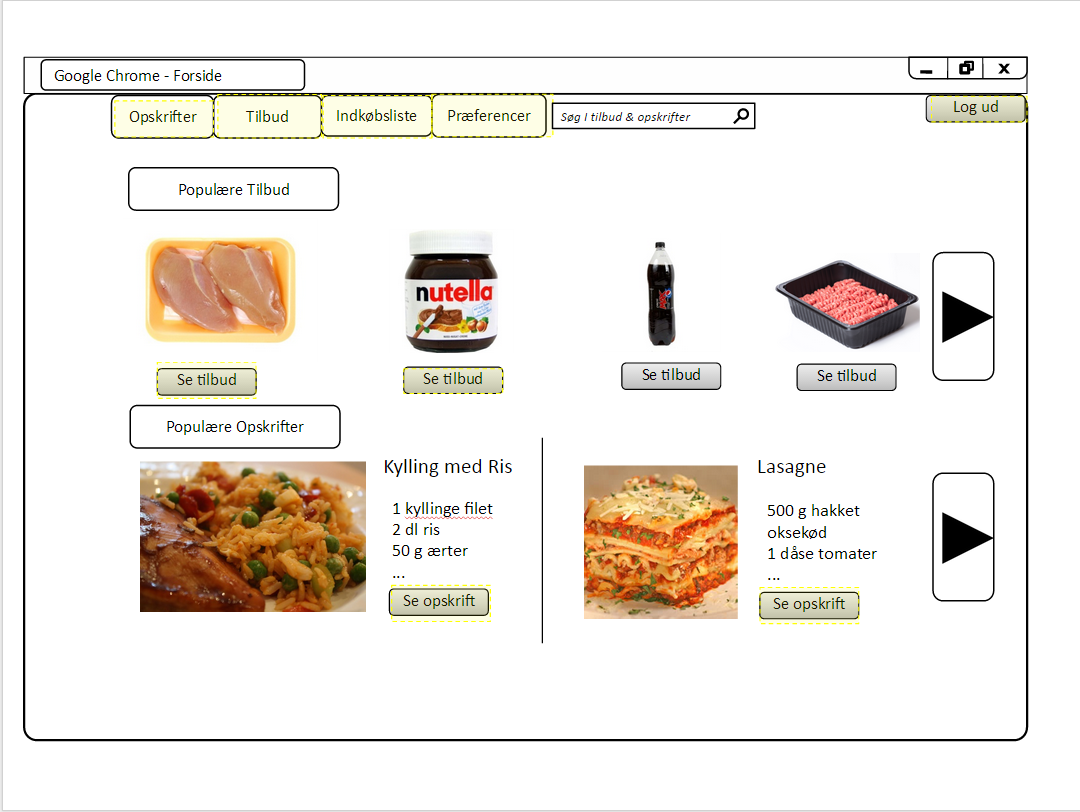
\includegraphics[width=0.66\textwidth]{images/Images/prototype-forside.PNG}
	\end{center}
	\vspace{-20pt}
	\caption{Forside fra Prototypen, der blev brugt i forbindelse med vores 2. runde af interviews}\label{ss:Prototype}
	\vspace{-20pt}
\end{wrapfigure}

Prototypen bruges i vores 2. runde af interviews, som har til formål at forstå hvilke funktionaliteter potentielle brugere ønsker i en løsning.
De interviewede bestod mest af unge personer i starten af tyverne, hvor af de fleste var studerende.
Dette valg blev taget da ud fra det første interview, blev det konkluderet at denne gruppe havde størst interesse i en løsning.
Interviewets fremgangsmåde kan findes på \fxnote{Indsæt kilde til interview fremgangsmøde.}

\fxnote{Er i tvivl om hvordan svarene skal sættes op. Skal vi bare bruge det corlin har skrevet og sætte ind, eller skal vi lave en overordnet gennemgang ligesom vi gjorde ved interview nummer 1? - Søren}

Ud fra denne undersøgelse står det nu klar at en løsning skal have følgende funktionaliteter:

\begin{itemize}
	\item Indkøbsliste integreret med tilbud.
	\item Oversigt over tilbud fra samtlige indkøbskæder.
	\item Opskrifter, som gør brug af tilbud.
	\item Mulighed for at vurdere opskrifterne og få anbefalet lignende.
	\item Valg af hvor man vil handle, hvilke madvarer man ikke vil spise osv.
	\item Deling af indkøbsliste med andre.
	\item Filtrering under opskrifter, så man kan se hvad man kan lave ud af f.eks. oksekød osv.
	\item Overvågning af varer, så man får en form for besked hvis noget kommer på tilbud en uge.
\end{itemize}

Der var også andre funktionaliteter som nogle af de adspurgte fandt relevante.
F.eks. blev en kalorietæller foreslået af en af de adspurgte, men dette vælges der at afgrænses fra, da det ikke hænger så godt sammen med resten af den meget tilbudsorienterede løsning.

Herudover gav de interviewende også forslag og råd angående hvilke funktionaliteter skulle være hvor i et desktop layout.
Disse forslag tages med i overvejelserne når brugergrænsefladen skal designes.
\fxnote{Indsæt evt. sætningen: En oversigt over alle de interviedes svar kan findes på bla bla bla i appendix. - Søren}
